\section*{Technik-Nomade}
\hypertarget{nomad}{}
\label{nomad}
\NewsAuthor{Horst JENS und Jonas SMEDEGAARD}

\textbf{Ein Lifestyle Bericht von \href{http://spielend-programmieren.at}{\textit{Horst JENS [5]}} \"uber \href{http://dr.jones.dk}{\textit{Jonas SMEDEGAARD [1]}}, einen Sysadmin aus D\"anemark der jahrelang freiwillig obdachlos lebte, aber niemals arbeitslos war und der dank Internet konsequent ortsunabh\"angig arbeitet.}
\begin{center}
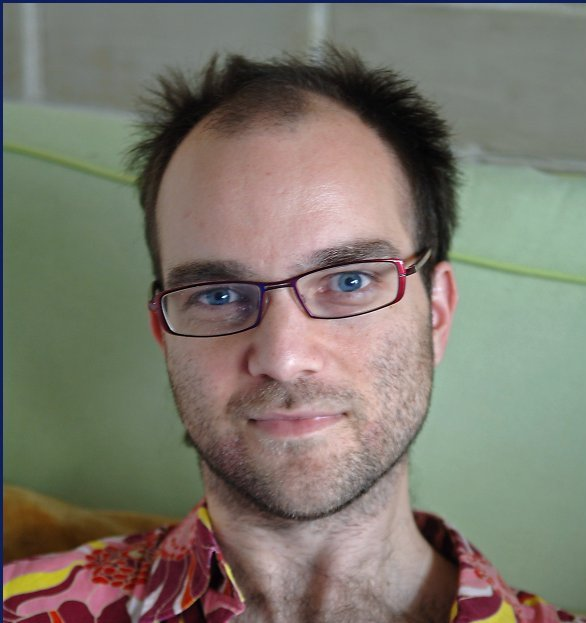
\includegraphics[width=5cm]{nomad/nomad-jonas.jpg}
\footnotesize{Jonas Smedegaard \href{http://dr.jones.dk}{{[}1{]}}, cc-by-sa}
\end{center}

'Herumzigeunern', 'obdachlos', 'Herbergssuche', 'nicht-sesshaft': Diese Worte haben im deutschen Sprachraum keinen guten Beigeschmack. Keinen festen Wohnsitz zu haben wird eher mit Armut als mit Freiheit assoziiert, eher mit Begriffen wie 'Versager' als mit 'Lifestyle'. Zumindest in meinem Freundes- und Bekanntenkreis erregt der Satz 'Ich weiß nicht wo ich morgen schlafen werde' Mitleid anstatt Neid.

Aus eigener Anschauung habe ich fast nur positive Erfahrungen mit kurzfristiger, freiwilliger Wohnungs-Ungewissheit gemacht: Eine Woche in England ausschließlich per \textit{Couchsurfing} unterwegs sein, als Jugendlicher mehrmals einen Monat lang per Interrail mit der Bahn herumfahren und in Fähren, Bahnhöfen, Felshöhlen und Gepäcknetzten schlafen, in Griechenland mit Schlafsack und Isomatte unterwegs sein: Aber immer mit der beruhigenden Gewissheit dass 'zu Hause' ein warmes Zimmer auf mich wartet, maximal ein, zwei Tagesreisen entfernt, komplett mit technischer und sozialer Infrastruktur. 

Umso mehr fasziniert es mich wenn ich Leute treffe die Obdachlosigkeit bewusst leben, nicht aus Not heraus oder als Urlaubsabenteuer, sondern sozusagen als Lebensabschnitt-Lifestyle: 

Jonas, einem System-Admin aus Dänemark, habe ich in Deutschland (bei einem \href{http://osdomotics.com}{\textit{OSDOmotics}}-Workshop\footnote{siehe Artikel \texttt{chemnitz}, RIS Journal 001, Seite \pageref{chemnitz})} im November 2013 kennen gelernt. Jonas sieht eine Spur unangepasst aus (so als ob er nicht oft Krawatten trägt) und hat eine sehr freundliche, extrovertierte Art. Speziell wenn es darum geht über die Vorteile von Linux oder freier Software zu reden wird er sehr enthusiastisch. 

\subsection*{Jonas}
Jonas wurde 1972 in Dänemark geboren, er beendete die (in Dänemark zehn-jährige) Grundschule aber flog zwei mal durch in der (drei-jährigen) Oberstufe. 1992, mit 20 Jahren,  \textit{'stopped trying to get an education'} gab er die Schule endgültig auf und ging seinen Interessen nach: Computern und Sozialarbeit.

Mit 19 Jahren (noch als Student) hatte er seinen ersten IT-Job: in einem 'Pre Press office' wurden Printings von Werbeagenturen druckfertig gemacht. Er war für die Vernetzung der Macintosh Computer zuständig. Im Gegensatz zu Windows PC's waren Macs zu dieser Zeit leicht vernetzbar, per Telefonkabel.

Mit einem \href{http://binx.com/}{\textit{Freund [2]}} welcher hobbymäßig Cartoons zeichnete erstellte Jonas erste Webseiten mit anklickbarer Grafik (image map) für den Netscape Navigator \footnote{aus diesem Browser ging später der populäre Mozilla Firefox hervor}. Jonas zog von zu Hause aus und wohnte in Kopenhagen und \href{https://en.wikipedia.org/wiki/Aarhus}{\textit{Aarhus}}. Er startete seine eigene IT-Firma \textit{Macværk} 1996 (später unbenannt in \textit{IT-guide dr. Jones}) als Einzelunternehmer.

Sein wichtigster Kunde war (und ist immer noch) die \href{http://kaospilot.dk/}{\textit{Kaospilot University [3]}} in Aarhus für die er als Systemadministrator arbeitete. Die Universität schickte ihre Studenten und Angestellten manchmal für ein Jahr zum Arbeiten ins Ausland, darunter auch Freunde von Jonas. Er versprach seinen Freunden, sie im Ausland zu besuchen.

Auf einer Reise in die Schweiz (Jonas begann sich mit Unix/Linux zu beschäftigen) wählte er sich vom Zug aus per Handy-Modem in einen Computer in Dänemark ein um seine Emails zu checken. Das war möglich weil er mit Linux im Terminal (Textmodus) arbeitete (ohne \textbf{GUI}) und daher nur wenig Bandweite brauchte. Dabei kam ihm zum ersten Mal die Erkenntnis das er von jedem Ort der Welt aus arbeiten konnte.

1998 besuchte er einen Freund der gerade ein Auslandsjahr in San Franzisko (USA) machte. Vor der Abfahrt stellte Jonas sicher keine offenen Rechnungen zu haben, kündigte seine Wohnung, aber nicht seinen Job. Auch von der USA aus arbeitete er weiter für seine Kunden in Dänemark. Der US-Aufenthalt war auf 3 Monate begrenzt, danach hatte er keine genauen Pläne... vielleicht weiter nach Kanada reisen. 

Distance working war damals gerade erst ein Schlagwort, alle Welt war der Meinung man müsste dafür erst mal schnelle ISDN-Verbindungen ausbauen. Jonas arbeitete per Dial-Up Modem und \href{http://de.wikipedia.org/wiki/Secure_Shell}{\textit{SSH}} Verbindung von San Franzisko aus um die Computer in Dänemark zu warten, sein Geld wurde weiterhin auf ein dänisches Konto gezahlt und er war weiterhin in Dänemark sozialversichert. Jonas musste nie um ein US-Arbeitsvisum ansuchen. Nur er selbst befand sich in den USA, seien Wertschöpfung erfolgte in Europa.

In dieser Zeit baute er einmal ordentlich Mist: er verwechselte bei einem Linux-Kommando ein \textbf{\textless} mit einem \textbf{\textgreater} während er die Datei \texttt{/etc/passwd} bearbeite. Dadurch wurde die Datei geschrieben anstatt gelesen und alle Studenten der Kaospilot University hatten keinen Zugang mehr zu ihren Emails. Während Jonas in San Francisco händeringend nach einer Lösung suchte (er bekam schließlich durch ein \href{https://en.wikipedia.org/wiki/Webmin}{\textit{Webmin}}-Web-Interface mit schlecht konfigurierter Security Zugang zu einem Backup-File) schrieb ihm ein (!) Student eine Email mit der Frage warum er seine E-mails nicht mehr checken kann. Der Rest der Studenten merkte nichts bis der Fehler behoben war oder beschwerte sich zumindest nicht. (Dabei spielt auch der Zeitunterschied zwischen Europa und USA eine Rolle). Seitdem schätzt Jonas die \textit{Pipe}\ (\textbf{$|$}) für Linux Kommandos.

%[{{ http://dr.jones.dk/images/mortenp199903.jpeg?250|Morten's Büroraum. Bildrechte: [[http://dr.jones.dk|Jonas Ssmedegaard]], Lizenz: [[http://creativecommons.org/licenses/by-sa/3.0/|cc-by-sa]]}}]
In Dänemark hatte sich Jonas für die Zeit seines Auslandaufenthaltes einen Büro-Raum in einem Internetcafe gemietet wo er seine Sachen einquartierte. Als er von den USA zurück kam plante er in diesem Büroraum (illegalerweise) auf dem Boden zu schlafen. Diese Pläne scheiterten daran dass das Internetcafe mittlerweile Pleite gegangen war, Jonas kam gerade noch rechtzeitig um seine Sachen abzuholen. Mangels Platz musste er einige alte, aber funktionierende Computer wegschmeissen, was ihm sehr leid tat. Schließlich erlaubte ihm sein Arbeitgeber, die Kaospilot University, einen Lagerraum zu benutzen. In diesem Lagerraum schlief Jonas auch. Einer seiner Freunde (Morten P.) hatte Mitleid und in der Universität einen festen Büroraum als Arbeitsplatz. Er ließ Jonas Nachts in diesem Büroraum schlafen -  unter dem Schreibtisch im Schlafsack. Sein Freund weckte ihn jeden Morgen um seinen Arbeitsplatz zu reklamieren.

Jonas hatte es nach eigenen Angaben zu dieser Zeit einfach satt ständig nach neuen Wohnungen (bzw. Lagerräumen) zu suchen die er doch nur für ein paar Monate behalten würde. Er beschloss daher bewusst auf Wohnungssuche zu verzichten und am Arbeitsplatz zu schlafen. 

Mit der Zeit wurde dies zu seinem Lifestyle. Er schlief oft bei verschiedenen Freunden. Da er nicht um 'Schlaferlaubnis für ein paar Tage' betteln wollte und seinen Freunden nicht lästig werden wollte unterließ er jede Vorausplanung seiner Schlafplätze sondern 'nahm jeden Tag so wie er kam'. Er wusste sprichwörtlich am Morgen nicht wo er am Abend schlafen würde...aber es machte ihm nichts aus. Wenn er einmal gar keinen Schlafplatz fand nahm er sich ein Hotelzimmer, eine Jugendherberge oder (weil billiger als ein Hotel) eine Schlafwagen-Bahnkarte für die Fahrt zwischen Aarhus und Kopenhagen. Der Zug fuhr nachts über ein Fährschiff, weshalb die Fahrt recht lange dauerte. 

%<html><div style="float:left; padding:5px"><a href="http://www.amazon.de/gp/product/B0069ZW3G4/ref=as_li_ss_il?ie=UTF8&camp=1638&creative=19454&creativeASIN=B0069ZW3G4&linkCode=as2&tag=spielendprogr-21"><img border="0" src="http://ws-eu.amazon-adsystem.com/widgets/q?_encoding=UTF8&ASIN=B0069ZW3G4&Format=_SL160_&ID=AsinImage&MarketPlace=DE&ServiceVersion=20070822&WS=1&tag=spielendprogr-21" ></a><img src="http://ir-de.amazon-adsystem.com/e/ir?t=spielendprogr-21&l=as2&o=3&a=B0069ZW3G4" width="1" height="1" border="0" alt="" style="border:none !important; margin:0px !important;" /></div></html>
%\begin{figure}

%width=\textwidth
\begin{center}
\href{http://goo.gl/9ENgMR}{
\includegraphics[width=\linewidth]{nomad/nomad-smoke.jpg} \\
\footnotesize{Smoke (Spielfilm). Bildrechte: Amazon Partner Programm [4]}}
%\footnotesize{\href{http://goo.gl/9ENgMR}{Smoke (Spielfilm). Bildrechte und Kauf: siehe Amazon.de [4]}}
\end{center}
%\caption{\footnotesize{Smoke (Spielfilm). Bildrechte und Kauf: siehe Amazon.de [4]}}
%\end{figure}


Duschen konnte er bei Freunden. Ein Problem war der Mangel an Kleidung: Er hatte drei verschiedene Sets von Kleidung, damit er immer ein Set waschen konnte. Sein Gepäck bestand aus einem Beutel mit den Kleidungs-Sets, Handtuch, Zahnbürste und Laptop.

In Waschsalons zog er sich zurück wenn er ein paar Momente 'alleine' sein wollte... Waschsalons sind besser geheizt als Bahnhöfe oder andere öffentliche Plätze, sind durchgehend geöffnet und weniger überfüllt. Mit Kopfhörern konnte er sich dort ruhig in eine Ecke setzten um zu computern, Musik zu hören oder Wäsche zu waschen.

Im Winter fand er ein Gentlemen’s Agreement mit einem Kaffeehausbesitzer in Aarhus. Dieser Mann war laut Jonas 'very laid back, like the owner in the film \href{http://goo.gl/9ENgMR}{\textit{Smoke [4]}}'. Unter anderem gab es in dem Kaffeehaus keine fixen Preise, sondern der Besitzer sagte jedem Kunden aus seiner Laune heraus wie viel er zu zahlen hat. 

Die Kunden liebten den schrulligen Besitzer. Während Jonas mit dem Besitzer tratschte (und von Gästen Whiskey spendiert bekam) fragte er wohin die Kellertüre führte. Ein Lagerraum den er für seine Sachen mieten konnte ? Ohne nachzudenken oder gar über einen Preis zu verhandeln gab ihm der Besitzer den Schlüssel...zum ganzen Kaffeehaus, nicht nur zum Lagerraum. Jonas musste für den Lagerraum (der zwar nicht geheizt war, aber ein Bett hatte) niemals etwas zahlen, nur einmal bat ihn der Cafehausbesitzer um einen Gefallen:
Eine Rechtsanwaltskanzlei hatte sich das Kaffeehaus für die Firmen-Weihnachtsfeier gemietet und der Besitzer wollte dass Jonas in die Party hineinplatzte mit der (wahren) Behauptung er wohne hier. 
Jonas tat ihm den Gefallen und ging einigen Jung-Anwälten auf die Nerven weil er sich großzügig vom Buffet bediente und mit den Sekretärinnen flirtete, aber schließlich trank er friedlich mit dem Chef der Anwaltskanzlei welcher ihn lustig fand.

Das Kaffeehaus wechselte den Besitzer und Jonas gab den Schlüssel zum Lagerraum zurück. 

Jonas lebte weiter sein Nomadenleben in Dänemark. Eine Wohnung vermisste er zu diesem Zeitpunkt nicht. Was ihm 'etwas' abging war 'die Bequemlichkeit mehr Kleider zu besitzen als man ständig herumtragen kann'. Im Herbst 1999 rief ihn eine japanische Bekannte an die er in Kalifornien kennen gelernt hatte. Ob er nach New York kommen wollte, das liege genau zwischen Kalifornien und Dänemark? Zuerst wollte er nicht, doch nach einer Woche nachdenken packte er seinen Laptop und flog nach New York. Dort wohnte er in einer Jugendherberge und dann bei Freunden von Freunden von Leuten die er zufällig kennen gelernt hatte. Zu dieser Zeit war \textbf{Couchsurfing} ein Begriff, noch keine Web Service.

%[{{ http://dr.jones.dk/images/me/jonas199903.jpeg?250|Jonas Housesitting. Bildrechte: [[http://dr.jones.dk|Jonas Ssmedegaard]], Lizenz: [[http://creativecommons.org/licenses/by-sa/3.0/|cc-by-sa]]}}]
Zu einer erhofften Romanze mit der japanischen Bekannten kam es nicht da sie nicht nur von ihrem Boy-Friend und einer Gruppe zusätzlicher Freunde, sondern auch von ihrer kleinen Schwester 'bewacht' wurde. Jonas fuhr zurück zu seiner nicht-existenten Wohnung nach Dänemark, sein mittlerweile trans-kontinentales Nomadenleben fortführend. In Dänemark lebte er zeitweise in der Wohnung seines Bruders, oder bei Freunden. Einmal betätigte er sich auch als 'house-sitter' und passte auf das Haus eines Bekannten auf. 

Er schlief unter anderem bei Kunden und einmal in einem Dachboden der Kaospilot University (wo er beim Aufstehen merkte das im Raum darunter eine Vorlesung stattfand).


Im Jahr 2000 (er wohnte gerade bei seinem Bruder) merkte er dass sein Bruder gerne mehr Privatsphäre hätte. Jonas wurde bewusst dass er nicht ewig bei Freunden und Verwandten leben konnte. Im Frühling 2000 lud Jonas die japanische Immer-noch-nicht-Freundin für einen Monat nach Dänemark ein. Als sie zusagte ging ihm auf dass er keine geeignete Wohnung sondern nur ein WG-Zimmer hatte und er seine Bekannte schlecht in Lagerräumen unterbringen konnte. Somit miete er kurzfristig einen zweiten Raum in der Wohngemeinschaft, sich vom obdachlosen Wohnraum-Schnorrer zum multiplen Zimmerbesitzer entwickelnd.

Zu seiner großen Freude kam die Japanerin ohne Boyfriend nach Dänemark, zu seinem großen Leidwesen brachte sie ihre kleine Schwester mit und er hatte kein einzige Mal die Gelegenheit mit der älteren Schwester alleine zu sein. Um das Masß voll zu machen wolten die beiden Mädchen ständig mit ihm Sight-seeing oder Aktivitäten machen  - stets alle zusammen. Die Situation wurde so unerträglich für ihn dass er sich schließlich äußert erratisch benahm, sich in Arbeit verkroch, von den japanischen Schwestern nichts wissen wollte und beide schlussendlich aus der Wohngemeinschaft (und damit aus Dänemark) hinauswarf.

Jahre später hat er sich für sein Verhalten entschuldigt und (der älteren Schwester) seine damaligen Gefühle gestanden. Sie dachte die ganze Zeit, er wäre homosexuell und deshalb nicht an ihr interessiert. 

Jonas miete sich in diversen Wohngemeinschaften ein und schließlich 2001 in einem \textbf{Hackerspace} in welchem Nachts elektronische Musik gemacht wurde und wo regelmäßig Konzerte stattfanden. In diesem Hackerspace (einer ehemaligen Fabrik) gab es einen Kontrollraum welcher gegen Funkenschlag geschützt war...ein \href{http://goo.gl/wfPa4p}{\textit{faradayscher Käfig}}. Jonas deponierte seine Sachen (und oft auch sich selbst) in diesem Kontrollraum. Laut seinen Angaben machte es ihm nichts aus in einem Käfig zu schlafen, aber die betrunkenen, lauten Konzertbesucher gingen ihm manchmal auf die Nerven.

Im September 2001 lernte Jonas seine jetzige dänische Freundin -Siri- kennen. Nach einer kurzen Beziehung mit ihr war er wieder Single. 2003 verließ Jonas Kopenhagen und zog in eine Ein-Zimmer Wohnung ein einem \href{https://en.wikipedia.org/wiki/Ecovillage}{\textit{Ecovillage (Ökodorf)}}. Sesshaft geworden merkte er dass ihm Siri (sie hatte inzwischen einen anderen Freund) fehlte und er wollte dass sie ihren damaligen Freund verlässt und zu ihm zog. Siri hatte zu diesem Zeitpunkt schon zwei Kinder und wollte zwar zu ihm ziehen, aber (aus für Jonas nicht ganz nachvollziehbaren Gründen) nicht in eine Ein-Zimmer-Wohnung. 2004 zogen Siri und Jonas endgültig zusammen - in eine größere Wohnung. Heute, 10 Jahre später, ist Jonas glücklich mit Siri zusammen und bewohnt mit ihr ein Haus auf einer kleinen dänischen Insel. Jonas hat nie aufgehört als selbstständiger IT-Administrator zu arbeiten und hat gute und langjährige Kunden. 


%[{{http://dr.jones.dk/images/jonas_og_siri.jpg?300|Jonas und Siri Bildrechte: [[http://dr.jones.dk|Jonas Ssmedegaard]], Lizenz: [[http://creativecommons.org/licenses/by-sa/3.0/|cc-by-sa]]}}]
\begin{center}
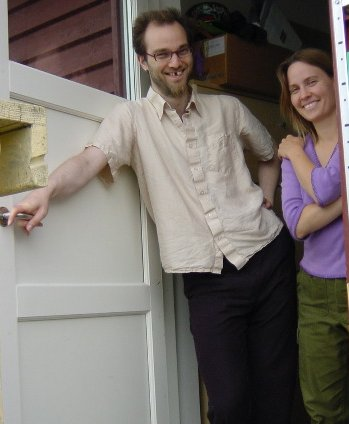
\includegraphics[width=5cm]{nomad/nomad-siri.jpg}
\footnotesize{Jonas und Siri in ihrem Haus. Bildrechte: \href{http://dr.jones.dk}{{[}1{]}}}
\end{center}

Obwohl mittlerweile ziemlich sesshaft und \emph{gut im Leben angekommen} hat Jonas sein Nomadentum nicht gänzlich abgelegt.

Immer wieder  zieht es ihn in die Ferne auf ausgedehnte internationale Vortragsreisen. Dort schläft er bei Fremden welche er nur von Online-Chats kennt, fliegt ohne Retourticket in fremde Länder für die er kein Visum hat um sich dort von Zufallsbekanntschaften am Flughafen zu Hackertreffen in noch fremdere Länder einladen zu lassen um schließlich bei Verwandten von Bekannten von Nachbarn von Leuten die er nicht kennt aufzuwachen und zu merken dass er weder Sprache noch primitivste örtliche Hygiene- oder Essgewohnheiten versteht. Jonas hält  Vorträge über Linux und Web-Technologie und lernt gerne neue Leute und fremde Kulturen kennen.

Und selbstverständlich betreut er seine dänischen Kunden weiter, egal wo er sich gerade befindet.

Jonas betreibt einen kleinen Blog auf \url{http://dr.jones.dk/} 

%[{{http://dr.jones.dk/images/fb/75864_10150123747827501_500217500_7805672_848154_n.jpg?250|Jonas auf einer Webtechnologiekonferenz in Asien. Bildrechte: [[http://dr.jones.dk|Jonas Smedegaard]] Lizenz: [[http://creativecommons.org/licenses/by-sa/3.0/|cc-by-sa]]}}]. 


\subsection*{Fachbegriffe}

~~~\textbf{Couchsurfing}: Eine besonders bei jungen Reiselustigen Leuten belibte Website, auf der man unkompliziert kostenlose Übernachtungsmöglichkeiten anbieten oder anfragen kann. Siehe \url{https://www.couchsurfing.org/}.

\textbf{GUI}: Graphical User Interface, (grafische Benutzerschnittstelle): wenn man einen Computer durch anklicken von Symbolen bedienen kann (z.B. Windows). Im Gegensatz dazu muss man im Textmodus Befehle eintippen, um z.B. alle Dateien in einem Verzeichnis zu sehen oder um z.B. ein Programm zu starten. \\

\textbf{Pipe}: (engl. f. Rohrleitung) Ein Umleitungsfunktion, die es ermöglicht dass der Output eines Befehls als Input eines anderen Befehls verwendet wird. Analog zur Anweisung: 'frag den Installateur welche Ersatzteile ihm fehlen und geh dann ins Lager und hole diese Ersatzteile'. Eine Pipe erzeugt man auf deutschen Tastaturen durch gedrückt halten der rechten Alt (Altgr) Taste und drücken der Taste links vom kleinen Ypsiolon... deren dritte Belegung ist ein senkrechter Strich, die Pipe. Mehr zum Thema erfahren Sie auf \href{http://wiki.ubuntuusers.de/Shell/Umleitungen}{der Wikiseite von \textit{ubuntuusers.de}}.

\textbf{Hackerspace} ein Raum wo gemeinschaftlich an Computer- und Hardwareprojekten geforscht und gearbeitet wird. In Wien z.B. das \href{http://metalab.at}{\texttt{metalab.at}} 

\subsection*{Podcast}
\begin{wrapfigure}{l}{2cm}
%\begin{center}

\includegraphics[width=2cm]{nomad/biertaucherlogo.png}
\end{wrapfigure}
%\end{center}
Horst erzählt über seine Begegnung mit Jonas im  \href{http://spielend-programmieren.at/de:podcast:biertaucher:2013:134}{\textbf{Biertaucherpodcast 134}: \texttt{goo.gl/WcUuX4}}
%\texttt{goo.gl/WcUuX4}}. 

\subsection*{Download, Feedback:}
\textbf{R.I.S.-Journal}, Ausgabe 001: \\
\href{http://spielend-programmieren.at/de:ris:001}{spielend-programmieren.at/de:ris:001}\\
\textbf{Download} Ordner, verschiedene Formate: \href{http://spielend-programmieren.at/risjournal/001/nomad}{\texttt{spielend-programmieren.at/\\risjournal/001/nomad}} \\
\textbf{Feedback} \Letter\ \texttt{dr@jones.dk} \\

\subsection*{Lizenz, Quellen:}

\begin{wrapfigure}{l}{2.0cm}
\begin{center}

\includegraphics[width=2cm]{nomad/ccbysa88x31.png}
\end{center}
\end{wrapfigure}
Dieses Material steht unter der Creative-Commons-Lizenz Namensnennung - Weitergabe unter gleichen Bedingungen 4.0 International. Um eine Kopie dieser Lizenz zu sehen, besuchen Sie \url{http://creativecommons.org/licenses/by-sa/4.0/deed.de}.

\textbf{Quellen}: \\
%\begin{itemize}
{[}1{]} \href{http://dr.jones.dk}{dr.jones.dk} \\
{[}2{]} \href{http://binx.com/}{binx.com} \\
{[}3{]} \href{http://kaospilot.dk/}{kaospilot.dk} \\
{[}4{]} \href{http://goo.gl/9ENgMR}{goo.gl/9ENgMR} \\ % amazon
{[}5{]} \href{http://spielend-programmieren.at}{spielend-programmieren}
